% Template for PLoS
% Version 1.0 January 2009

\documentclass[10pt]{article}

% amsmath package, useful for mathematical formulas
\usepackage{amsmath}
% amssymb package, useful for mathematical symbols
\usepackage{amssymb}
\usepackage{tabularx}

% graphicx package, useful for including eps and pdf graphics
% include graphics with the command \includegraphics
\usepackage{graphicx}

% Need to have subfigures
\usepackage{subcaption}
\pdfpagebox5

% cite package, to clean up citations in the main text. Do not remove.
\usepackage{cite}

\usepackage{color}
\usepackage[squaren]{SIunits} 
%\usepackage{units}

% Use doublespacing - comment out for single spacing
%\usepackage{setspace} 
%\doublespacing

\usepackage{pgfplots}
\usepgfplotslibrary{dateplot}

% Text layout
\topmargin 0.0cm
\oddsidemargin 0.5cm
\evensidemargin 0.5cm
\textwidth 16cm 
\textheight 21cm

% Bold the 'Figure #' in the caption and separate it with a period
% Captions will be left justified
\usepackage[labelfont=bf,labelsep=period,justification=raggedright]{caption}

% Use the PLoS provided bibtex style
\bibliographystyle{plos2009}

% Remove brackets from numbering in List of References
\makeatletter
\renewcommand{\@biblabel}[1]{\quad#1.}
\makeatother


% Leave date blank
\date{}

\pagestyle{myheadings}
%% ** EDIT HERE **

%% ** EDIT HERE **
%% PLEASE INCLUDE ALL MACROS BELOW
\usepackage[printonlyused]{acronym}
\usepackage{multicol}

%% END MACROS SECTION

\begin{document}

% Title must be 150 characters or less
\begin{flushleft}
{\Large
\textbf{Modeling Poplar Growth as a Short Rotation Woody Crop for Biofuels}
}
% Insert Author names, affiliations and corresponding author email.
\\
Quinn Hart$^{1,\ast}$,
Olga Prelipova$^{2}$,
Justin Merz$^{1}$,
Peter Tittmann$^{3}$, 
Bryan Jenkins$^{4}$
\\
$^{\textbf{1}}$ Department of Land, Air, and Water, University of California, Davis, USA
$^{\textbf{2}}$ Department of Computer Science, University of California, Davis, USA
$^{\textbf{3}}$ Department of Forestry, University of California, Berkeley, USA
$^{\textbf{4}}$ Energy Institute, University of California, Davis, USA
\\
%\\textbf{3} Author3 Dept/Program/Center, Institution Name, City, State, Country
$\ast$ E-mail: qjhart@ucdavis.edu
\end{flushleft}

% Please keep the abstract between 250 and 300 words
\section*{Abstract}

\acp{SRWC} have been proposed in an number of studies as a good
potential feedstock for a cellulosic derived biofuel.  The ability to
accurately predict the growth and yield of \ac{SRWC} under various
environmental conditions is an important step in the development of
energy system that can incorporate these feedstocks.  An important
aspect of \acp{SWRC} is how coppicing is often used in the management
of a plantation.  There have been a number of studies that have used
the \ac{3pg} as a model for predicting growth and yields. 

In this study, the \acf{3pg} model was modified for \ac{SRWC} with the
inclusion of a coppicing model.  We parameterized the model some
previously published results for modeling poplar growth, and then
applied this model to a set of field tests measuring poplar growth and
yields in a coppiced regime.
 
% Please keep the Author Summary between 150 and 200 words
% Use first person. PLoS ONE authors please skip this step. 
% Author Summary not valid for PLoS ONE submissions.   
%\section*{Author Summary}

\section*{Introduction}

The goals of this research were to develop modifications to the
\ac{3pg} model to allow for an accurate representation of growth of
\ac{SRWC}, particularly poplar over a range of environmental
conditions and to validate the model compared to various field trials.

We are developing and testing species parameters to use the \acf{3pg}
model as a means to estimate poplar yields, primarily for the Pacific
Northwest.  Modeling the physiological growth is advantageous because
it allows variation of poplar species parameters and management
practices.  Because it is a canopy carbon balanced model, allocations
for both above and below ground biomass can be tracked for studies
like life-cycle analysis.

The original \ac{3pg} model does not include coppicing as a management
practice, which is problematic as it cannot reasonably account for
post-coppicing regrowth.  The extended model includes coppicing with a
general model that allows a monthly growth contribution from an
existing root mass.  The model specifies a relatively small
contribution of above-ground growth from the accumulated root mass
after coppicing in order to initiate the next cycle of production.

The primary modification is the inclusion of a coppicing model for the
prediction of biomass production over the course of a number of
coppicing cycles.  The coppicing model introduced is a simple extension
that models the sprouting of the coppice, contribution to growth from
the existing root system, and modifications to the allocation of
resources based on the coppicing.

We parameterized the model some previously published results for
modeling poplar growth, and then applied this model to a set of field
tests measuring poplar growth and yields in a coppiced regime.

\newcommand{\pop}{\textit{Populus} }

%\begin{multicols}{3}[\section*{Acronyms}]
%\addcontentsline{toc}{section}{Acronyms}
%{\normalsize
%\raggedright
%\setlength{\columnseprule}{1pt}
%\begin{acronym}
\acrodef{gbsm}[\textsc{GBSM}]{Geospatial Bioenergy Systems Model}
\acrodef{3pg}[\textsc{3PG}]{Physiological Principles in Predicting Growth}
\acrodef{dW}[\ensuremath{\Delta W}]{Total Monthly Growth}
\acrodef{GIS}[\textsc{GIS}]{Geographical Information System}
\acrodef{SRWC}[\textsc{SRWC}]{Short Rotation Woody Crops}
\acrodef{NPP}[\ensuremath{NPP}]{Net Primary Productivity}
\acrodef{LAI}[\ensuremath{LAI}]{Leaf Area Index}
\acrodef{LAIt}[\ensuremath{LAI_{T}}]{Target Leaf Area Index}
\acrodef{RP}[\ensuremath{RP}]{Root Productivity}
\acrodef{NPPdef}[\ensuremath{NPP_{def}}]{$NPP$ deficit}
\acrodef{NPPt}[\ensuremath{NPP_{T}}]{$NPP$ if $LAI = LAI_{T}$}
\acrodef{dRres}[\ensuremath{\Delta R_{res}}]{Residual root contribution}
\acrodef{pRx}[\ensuremath{p_{R\%x}}]{Maximum root \%}
\acrodef{Rdp}[\ensuremath{R_{\Delta\%}}]{Root contribution}
\acrodef{W}[\ensuremath{W}]{Total plant mass}
\acrodef{WR}[\ensuremath{W_R}]{Total root mass}
\acrodef{fAge}[\ensuremath{f_{age}}]{age Growth Limiter}
\acrodef{fR}[\ensuremath{f_R}]{Root conversion efficiency}
\acrodef{fi}[\ensuremath{f_i}]{Generic growth limiters}
%\end{acronym}
%}
%\end{multicols}

% You may title this section "Methods" or "Models". 
% "Models" is not a valid title for PLoS ONE authors. However, PLoS ONE
% authors may use "Analysis" 
\section*{Models}

Figure~\ref{fig:growth-model} shows and overview of the main
components used in the development of the poplar growth model. The
model is based primarily on the \acf{3pg} model~\cite{Landsberg1997,
  landsberg2010physiological}, with modifications for coppicing with
\ac{SRWC}.

\begin{figure}[!ht]
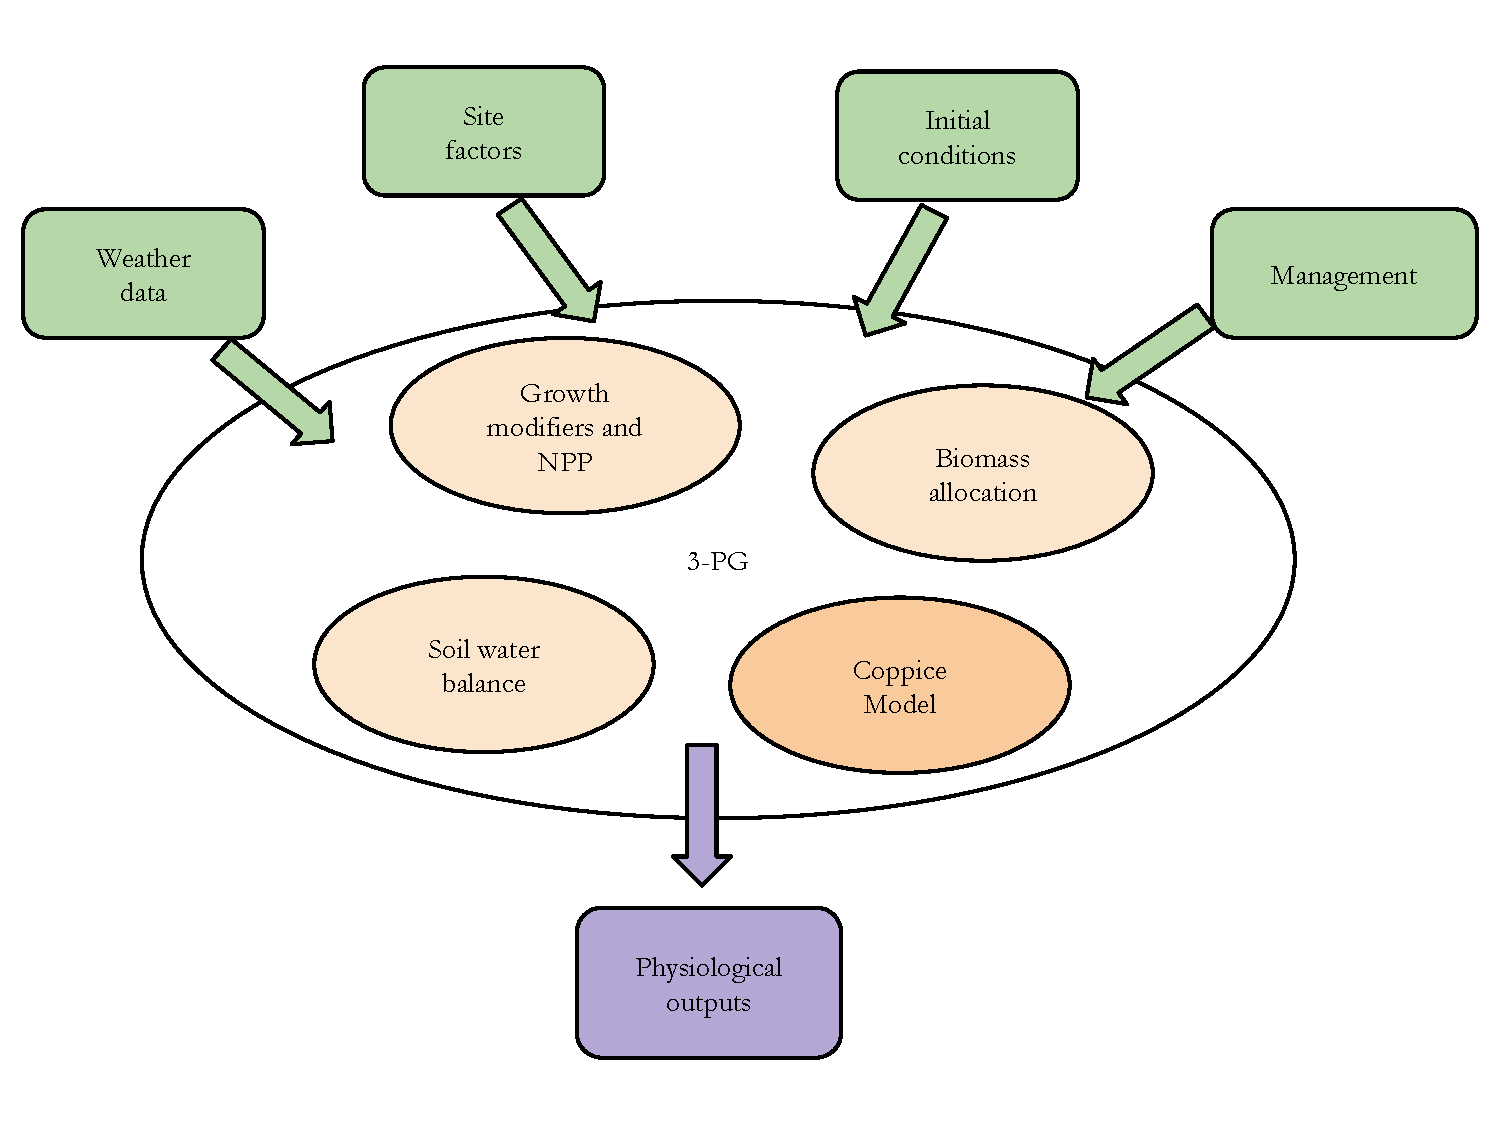
\includegraphics[width=0.5\linewidth]{model_overview}
\caption{ \textbf{\ac{3pg} Overview.}}
\label{fig:growth-model}
\end{figure}

The \ac{3pg} model takes as inputs weather data, site factors, initial
conditions, management practices, and species information.  The model
typically runs at a monthly timestep. At each step the physiological
parameters are calculated and carried forward to the next month. Input
weather parameters are specified at the same monthly timestep, and
additional management parameters, such as irrigation scheduling, and
when the poplar is coppiced are also be included.

The physiological components of the \ac{3pg} model comprises of
sub-modules for estimating growth modifiers and \ac{NPP}, biomass
allocation, and soil water balance.  We have added an additional
module for regrowth after coppicing.  In general, the \ac{3pg} model
works by predicting expected productivity based on input weather
conditions, soil parameters and their interaction with the species
being modeled.  The productivity is basically a computed maximum value
with a number of multiplicative limiters based on the plants response
to temperature, water availability, fertility, and other species
dependent processes.

%\subsubsection*{Poplar Hybrids with \ac{3pg}}

There have been a few studies have been reported for modeling poplar
using the \ac{3pg} model~\cite{Amichev2010,Headlee2012}.
Headlee~\cite{Headlee2012} in particular, developed a set in \pop
parameters from a set of both laboratory and field studies.  The
inputs used in this study draw from these studies to parameterize the
growth of a representative hybrid poplar.  As will be discussed in
Section~\ref{sec:validation}, different \pop clones can vary
considerably in their growth patterns.  The following tables summarize
the base parameters used for the generic \pop model, for this study.

\begin{table}[!ht]
\caption{\textbf{\ac{3pg} Model Tree Parameters}}
%\begin{tabular}{|c|c|c|}
\hline
Parameter & Source & value\\
\hline
\multicolumn{3}{|c|}{Greenwood Plantation Values}\\
type &  & ,\\
StockingDensity &  & 3587,\\
SeedlingMass &  & 0.0004,\\
pS &  & 0.1,\\
pF &  & 0,\\
pR &  & 0.9,\\
\hline
\multicolumn{3}{|c|}{Soil information based on current location}\\
maxaws &  & -1,\\
swpower &  & -1,\\
swconst &  & -1,\\
\hline
\multicolumn{3}{|c|}{ Weather Parameters}\\
month &  & -1,\\
tmin &  & -1,\\
tmax &  & -1,\\
tdmean &  & -1,\\
ppt &  & -1,\\
rad &  & -1,\\
nrel &  & -1,\\
daylight &  & -1,\\
\hline
\end{tabular}

\begin{tabularx}{\linewidth}{|c|X|c|}
  \hline
  Parameter & Source & Value\\
  \hline
  \acs{k}  & \acf{k} & 0.5\\
  fullCanAge [yr] & Year where tree reaches full Canopy Cover. & 0  \\
  kG \reciprocal\kilo\pascal & Determines the response of the canopy conductance to the vapor pressure deficit. & 0.5\\
  alpha [\kilogram\mole] & Canopy quantum efficiency. & 0.06\\
  \hline
  \acs{fT} [frac] & The parameters specifing limitations from ambient temperature. & \\
  $mn_{\acs{fT}}$ [\Celsius] & The minimum temperature for respiration & 5\\
  $opt_{\acs{fT}}$ [\Celsius] & The optimum temperature for respiration & 20\\
  $mx_{\acs{fT}}$  [\Celsius] & The maximum temperature for respiration & 40\\
  \hline
  \acs{BLcond} [\reciprocal\meter] & Canopy boundary layer conductance. Used in the calcuation of transpiration & 0.2\\
  \hline
  \acs{fAge} [frac] & Specifies the growth limiter as a function of the tree age.  This is a time dependant parameter. Specified with 4 parameters. & \\
  $f0_{\acs{fAge}}$ &  Value for \acs{fAge} at Initial Time & 1\\
  $f1_{\acs{fAge}}$ & Value for \acs{fAge} at Infinite Time & 0 \\
  $tm_{\acs{fAge}}$ [y] & Time in years where value is the average of $f0$ and $f1$ & 47.5\\
  $n_{\acs{fAge}}$ & $n>=1$ Parameter specifing the rate of change around tm.  n=1 is approximately a linear change, as n increases, change becomes more localized around tm. & 3.5\\
  \hline
   $fN0$ [frac] & Used in the calculation of the nutritional modifier,$fNutr$.  $fNutr$ ranges from [$fNO$,1) based on the fertility index which ranges from 0 to 1.  When $fN0=1$ indicates $fNutr=1$ & 1\\
   \hline
   \acs{SLA} [$\square\meter\per\kilogram$] & \acf{SLA}.  Defined as a function of the tree age.  Used in the calculation of LAI. &\\
   $f0_{\acs{SLA}}$ & \acs{SLA} at initial time & 10.8\\
   $f1_{\acs{SLA}}$ & \acs{SLA} at infinite timestep & 10.8\\
   $tm_{\acs{SLA}}$ [y] & Time in years where value is the average of $f0$ and $f1$ & 1\\
   $n$  & $n>=1$; Parameter specifing the rate of change around $tm$.  $n=1$ is approximately a linear change, as n increases, change becomes more localized around $tm$. & 2\\
   \hline
   $Cond$ [$\meter\per\second$] &  Canopy Conductance.  Along with a Physiological modifer, specifies the canopy conductance.  Used in calculation of transpiration & \\
   $mn_{Cond}$ & Minimum value, when $lai=0$ & 0.0001\\
   $mx_{Cond}$ & Maximum value & 0.02\\
   $lai_{Cond}$ [$\square\meter\per\square\meter$] & \ac{LAI} where parameter reaches a maximum value. & 3.33\\
 \hline
 $Intcptn$ [frac] & Rainfall interception fraction.  A linear function w.r.t. \ac{LAI} & \\
  $mn_{Intcptn}$ & Minimum value, when lai=0 & 0\\
  $mx_{Intcptn}$ & Maximum value & 0.15\\
  $lai_{Intcptn}$ [$\square\meter\per\square\meter$] & \ac{LAI} where parameter reaches a maximum value. & 5\\
 \hline \hline
 y & Assimilation use efficiency.  Used in calculation of the NPP. & 0.47\\
 \hline 
\end{tabularx}


\begin{flushleft}The table shows the data sources used for the
  modeling of the potential Growth model for poplar.
\end{flushleft}
\label{tab:3pg-tree}
 \end{table}

\subsection*{Coppicing Model}
\label{sec:coppicing-model}

The original \ac{3pg} model allocates the monthly productivity from
transpiration of the trees into the creation of new roots, stems and
foliage.  In the standard \ac{3pg} model, the amount allocated to
roots is basically a constant allocation, potentially with a modifier
due to the plants fertility stress. The amount allocated to the
foliage and stems is dependent on the age and size of the trees.  In a
\ac{SRWC} however, coppicing the trees during harvesting introduces a
situation where the stem and foliage are removed, but the root ball
remains.  Because the original model derives it's production from
transpiration, the \ac{3pg} model has no mechanism to increase to
start re-growth from this situation.  In addition the model does not
moderate the allocations based on the abrupt changes in the allocation
in the plant.

\begin{figure}[!ht]
\begin{subfigure}[b]{.1125\linewidth}
\centering
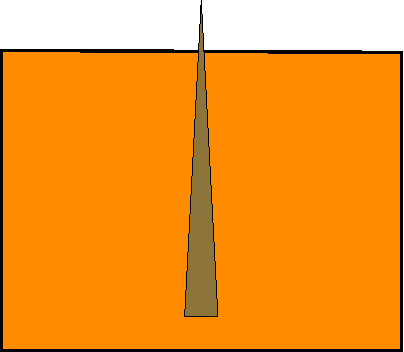
\includegraphics[width=1.0\linewidth]{img/tree_pics_1}
\caption{}  %\caption{planting}
\label{fig:grow_1}
\end{subfigure}
\begin{subfigure}[b]{.1125\linewidth}
\centering
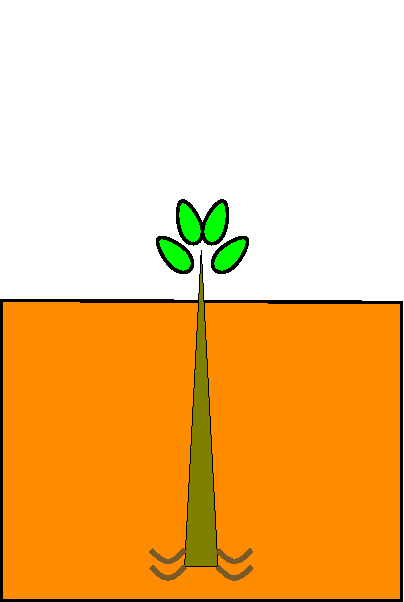
\includegraphics[width=1.0\linewidth]{img/tree_pics_2}
\caption{}  %\caption{sprout}
\label{fig:grow_2}
\end{subfigure}
\begin{subfigure}[b]{.1125\linewidth}
\centering
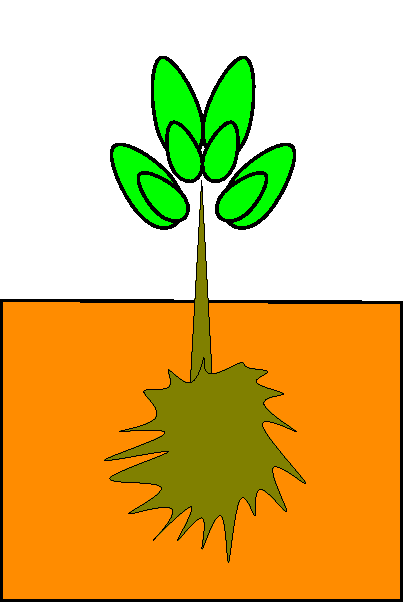
\includegraphics[width=1.0\linewidth]{img/tree_pics_3}
\caption{}  %\caption{growth}
\label{fig:grow_3}
\end{subfigure}
\begin{subfigure}[b]{.1125\linewidth}
\centering
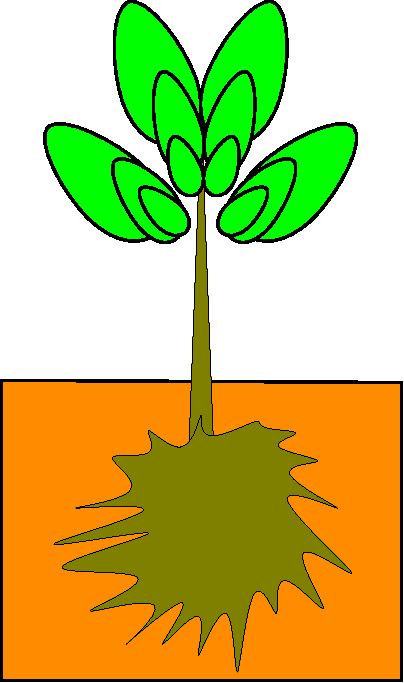
\includegraphics[width=1.0\linewidth]{img/tree_pics_4}
\caption{}  %\caption{maturity}
\label{fig:grow_4}
\end{subfigure}
\begin{subfigure}[b]{.1125\linewidth}
\centering
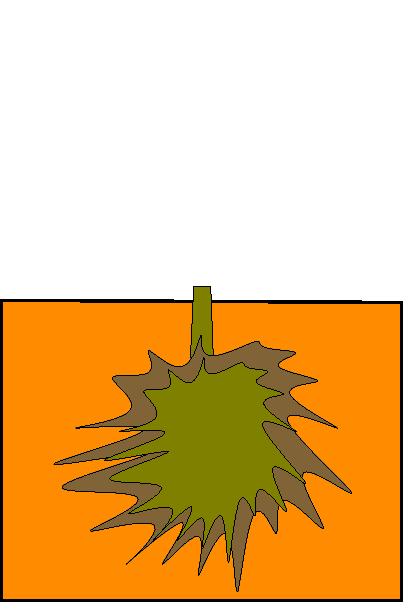
\includegraphics[width=1.0\linewidth]{img/tree_pics_5}
\caption{}  %\caption{coppiced}
\label{fig:grow_5}
\end{subfigure}
\begin{subfigure}[b]{.1125\linewidth}
\centering
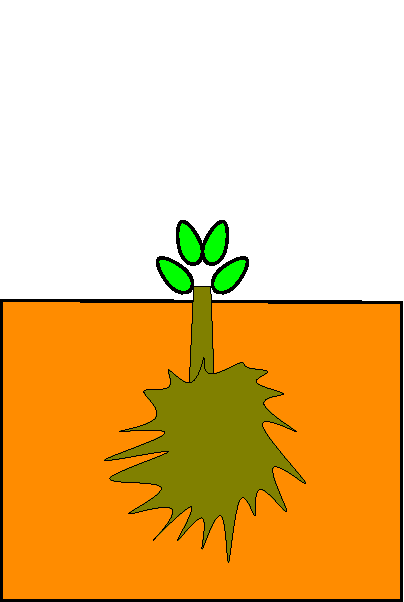
\includegraphics[width=1.0\linewidth]{img/tree_pics_6}
\caption{}  %\caption{resprouting}
\label{fig:grow_6}
\end{subfigure}
\begin{subfigure}[b]{.1125\linewidth}
\centering
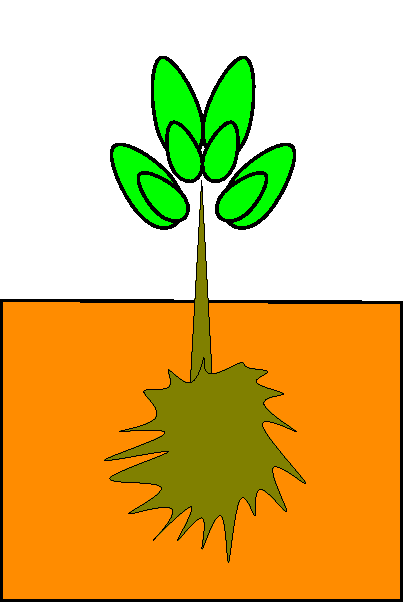
\includegraphics[width=1.0\linewidth]{img/tree_pics_7}
\caption{}  %\caption{regrowth}
\label{fig:grow_7}
\end{subfigure}
\begin{subfigure}[b]{.1125\linewidth}
\centering
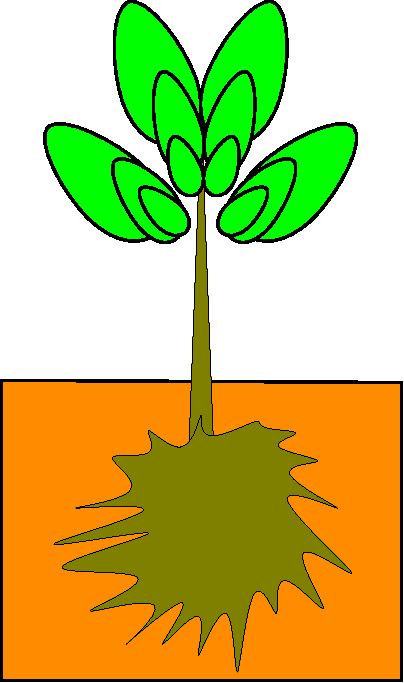
\includegraphics[width=1.0\linewidth]{img/tree_pics_4}
\caption{}  %\caption{next harvest}
\label{fig:grow_8}
\end{subfigure}
\caption{ \textbf{Poplar \ac{SRWC} growth.} The growth stages for poplar
  grown as an \ac{SRWC} with one coppicing cycle shown. }
\label{fig:grow}
\end{figure}

Figure~\ref{fig:grow} shows the typical growth of a poplar planted as
a \ac{SRWC}.  Poplars are generally propagated via cuttings of bare
poplar stem, mostly under the soil,~(Figure~\ref{fig:grow_1}).  The
cutting provides energy for the establishment of the seedling via buds
above and below the surface~(Figure~\ref{fig:grow_2}). As the poplar
matures, it is the productivity provided by the plant's transpiration
that provides for growth.  This includes the establishment of the root
ball~(Figure~\ref{fig:grow_3}).  By the time the poplar is ready for
coppicing~(Figure~\ref{fig:grow_4}), the plants are well established.

After coppicing, there is a surfeit of root mass, and no foliage to
provide photosynthetic based productivity to the
tree~(Figure~\ref{fig:grow_5}).  However, a portion of the root mass
is available as a production source for the tree.  Sometime later, the tree
resprouts with the root ball providing initial energy for the
reestablishment of seedlings~(Figure~\ref{fig:grow_6}) which then
leads through the maturation of the poplar, ready for the next
harvest~(Figures~\ref{fig:grow_7} and~\ref{fig:grow_8}).

Modeling the growth of the \ac{SRWC} then becomes a task of determining
the size and timing of the regrowth from the existing root mass.

We have developed a simple root interaction system added to the
\ac{3pg} model to model the behavior both of the post-coppiced
situation as well as the initial planting of the cutting. At any given
timestep the model augments the productivity from the plant's
transpiration with an additional production from utilization of
reserves with in the root mass.  Under normal conditions, this
augmentation is zero, however, with the initial planting of the
cutting, or after a coppicing event, this augmentation is used to add
foliage to the tree and start transpiration based production again.

An overview of the model is shown in figure~\ref{fig:coppice}.  Three
species specific parameters control the coppicing model.  Combined
with the input weather, and some parameters in the \ac{3pg} model,
these control the extent and the timing of the regrowth from the
coppiced plant.

\begin{figure}[!ht]
  \centering
\begin{subfigure}[b]{.2\linewidth}
  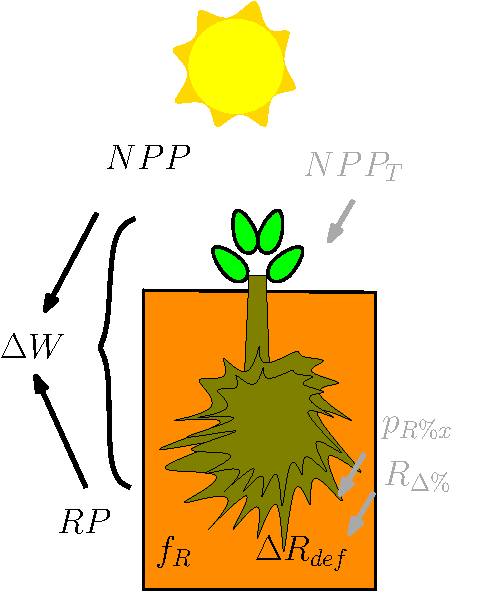
\includegraphics[width=1.0\linewidth]{img/tree_pics_10}
  \caption{Parameters}
  \label{fig:coppice-img}
\end{subfigure}
\quad
\begin{subtable}[b]{.75\linewidth}
\begin{align}
\acs{dW}=\acs{NPP}+\acs{RP} \\
\acs{RP} = \begin{cases} 0 & \acs{NPPdef} <=0 \\
\acs{fR} ~ min (\acs{dRdef} ,\acs{NPPdef}) & \acs{NPPdef} > 0  
\end{cases} \\
\acs{NPPdef} = \acs{NPPt}-\acs{NPP} \\
\acs{dRdef} = \acs{WR}(\acs{WR}/\acs{W} - \acs{pRx})\acs{Rdp}
\end{align}
\caption{Model Definition}
\end{subtable}
\caption{\textbf{Coppice Model Overview}}
  \label{fig:coppice}
\end{figure}

The model is designed to integrate easily into that existing \ac{3pg}
equations, with limited modifications.  To that end, at each monthly
timestep, the model allocates it's productivity as before.  The only
difference being that \acf{dW} is now the sum of the \acf{NPP} and an
additional \acf{RP}.  The contribution from \ac{RP} however, is
dependent on the weather, the state of the plant, and some parameters
defining the root mass characteristics. 

The contribution \ac{RP} is affected by the potential of a plant to
grow under the current weather conditions, as defined by the potential
productivity of the plant.  \ac{NPPt} defines a target productivity
within a given timestep.  This target can in turn be defined with
\acs{LAIt}, a target \ac{LAI} which may or may not be realized by
tree's current distribution .  The \acs{LAIt} parameter can be thought
of as defining a minimum operational \acs{NPP} which the plant
attempting to reach.

\acs{LAIt} can vary from 0 and greater.  A value of 0 indicates no
root contribution, where higher values indicate contribution from the
roots even as the plant is producing higher values for \acs{NPP} from
it's foliage.

This affects the timing of the root contribution, because the
\ac{NPPt} is affected by the current weather conditions.  If those
conditions are not conducive to plant transpiration, then \ac{NPPt}
is low, and resources are not allocated for growth.

\ac{NPPdef} is then defined as the difference between the \ac{NPPt}
and \ac{NPP}. \ac{NPPdef} defines a maximum contribution from the
roots to the overall plant growth.  The actual contribution is also
limited by the amount of energy available in the root mass at any
given timestep.

As described above, \ac{3pg} model defines a root allocation
parameter, \acs{pRx}, which defines the root size with respect to the
entire plant size.  After coppicing, the root mass is larger then
\acs{pRx}.  Some amount of that extra root mass will be made available
for \ac{RP}.  The parameter, \ac{Rdp}, (ranging from 0 to 1), defines
what fraction this surplus root mass can contribute to \ac{RP} in a
given timestep.  A value of 0 indicates no root contribution for
regrowth, higher values indicate more potential growth available to
the plant at each timestep.

Finally, the parameter \acf{fR}, ranging from 0 to 1, determines the
efficiency of the contribution, in effect, determining the fraction of
new mass of growth, to loss of root mass.  \acs{fR} is multiplied with
the available root mass to determine \ac{RP}.

In poplar plantations, initially planted with cuttings, original
growth is modeled the same way.  A different set of parameters for
\ac{LAIt},\ac{Rdp}, and \acs{fR} can be used for the cutting and the
post-coppiced trees.

Figures~\ref{fig:date},~\ref{fig:rdp} and~\ref{fig:lai} illustrate the
effect of these parameters on the expected plant growth.  For these
examples, the climatic parameters described in
Figure~\ref{fig:weather} were used.  The plants were also never
limited by water availability.

\begin{figure}
  \centering
  \begin{tikzpicture}
  \begin{axis}[
    no markers,
    width=\linewidth,
    height=2in,
    date coordinates in=x,
    xticklabel={\month},
    ylabel style={align=center}, ylabel=Rad {$[MJ/day]$}; Temp {$[C]$}\\ Daylight {$[hr]$},
    stack plots=false,
    bar width=2pt,
    legend entries={$T_n$,$T_x$,$R$,$Hrs$},
    legend style={at={(0.4,1.03)},anchor=south},
    legend columns=4,
    %legend to name = temp
    % legend style={
    % at={(0.5,-0.3)},anchor=north,legend columns=-1}
    ]
    \addplot+[color=yellow] table [x=date, y=tmin, col sep=comma] {coppice/weather.csv};
    \addplot+[color=red ] table [x=date, y=tmax, col sep=comma] {coppice/weather.csv};
    \addplot+[ybar, color=blue, fill=blue] table [x=date, y=rad, col sep=comma] {coppice/weather.csv};
    \addplot+[ybar, color=green, fill=green] table [x=date, y=daylight, col sep=comma] {coppice/weather.csv};
    
  \end{axis}
  \begin{axis}[
     no markers,
     width=\linewidth,
     height=2in,
     date coordinates in=x,
  %   ylabel=PPT [mm],
     axis y line=right,
     axis x line=none,
  %   % ylabel style={yshift=10pt},
     legend entries={$PPT$},
     legend style={
        at={(.7,1.03)},
        anchor=south},
     %legend to name = ppt,
     ylabel style={align=center}, ylabel=Precip {$[mm]$},
     ]
    \addplot+[color=black] table [x=date, y=ppt, col sep=comma] {coppice/weather.csv};
   \end{axis}
\end{tikzpicture}
%\ref{temp}

  \caption{Input example weather data, replicating conditions around
    Corvallis, OR}
  \label{fig:weather}
\end{figure}

A plant parameterized with $\ac{Rdp}=1$, $\acs{fR}=1$ and
$\acs{LAIt}=100$ will reallocate the maximum resources back into plant
growth as fast as possible.  This is an illustrative example to show
the affect of the season on the modeled regrowth.
Figure~\ref{fig:date} shows the response of this plant for various
coppicing dates.  In this example, the

\begin{figure}
  \centering
  \pgfplotsset{
      no markers,
      width=\linewidth,
      height=0.25\linewidth,
      every axis plot/.append style={line width=1pt},
      date coordinates in=x,
      xmin={2016-02-15},
      xmax={2019-10-15},
      xtick={2016-06-15,2016-09-15,2016-12-15,
      2017-03-15,2017-06-15,2017-09-15,2017-12-15,
      2018-03-15,2018-06-15,2018-09-15,2018-12-15,
      2019-03-15,2019-06-15,2019-09-15},
      x tick label style={rotate=45, anchor=east},
      xticklabels={Y2-06,Y2-09,Y2-12,
      Y3-03,Y3-06,Y3-09,Y3-12,
      Y4-03,Y4-06,Y4-09,Y4-12,
      Y5-03,Y5-06,Y5-09},
      ymin=0,ymax=60,
      ytick={20,40},
      yticklabels={20,40},
}
  \begin{tikzpicture}
    \begin{axis}[
      name=feb,
      legend entries={Stem,Root,Foilage},
      legend style={
        at={(0.5,1)},anchor=south,legend columns=-1,yshift=1pt},
      xticklabels=\empty,
      ]
      \node[right] at (axis cs:{2016-02-15},50) {Y3-02};
      \addplot+[color=brown] table [x=date, y=m02f1, col sep=comma] {coppice/hart12coppice-coppice-ws.csv};
      \addplot+[color=red] table [x=date, y=m02f1, col sep=comma] {coppice/hart12coppice-coppice-wr.csv};
      \addplot+[color=green] table [x=date, y=m02f1, col sep=comma] {coppice/hart12coppice-coppice-wf.csv};
    \end{axis}
    \begin{axis}[
      name=may,
      at={(feb.below south west)},yshift=5pt,
      anchor=north west,
      xticklabels=\empty,
      ]
      \node[right] at (axis cs:{2016-02-15},50) {Y3-05};
      \addplot+[color=brown] table [x=date, y=m05f1, col sep=comma] {coppice/hart12coppice-coppice-ws.csv};
      \addplot+[color=red] table [x=date, y=m05f1, col sep=comma] {coppice/hart12coppice-coppice-wr.csv};
      \addplot+[color=green] table [x=date, y=m05f1, col sep=comma] {coppice/hart12coppice-coppice-wf.csv};
    \end{axis}
    \begin{axis}[
      name=aug,
      at={(may.below south west)},yshift=5pt,
      anchor=north west,
      xticklabels=\empty,
      ]
      \node[right] at (axis cs:{2016-02-15},50) {Y3-08};
      \addplot+[color=brown] table [x=date, y=m08f1, col sep=comma] {coppice/hart12coppice-coppice-ws.csv};
      \addplot+[color=red] table [x=date, y=m08f1, col sep=comma] {coppice/hart12coppice-coppice-wr.csv};
      \addplot+[color=green] table [x=date, y=m08f1, col sep=comma] {coppice/hart12coppice-coppice-wf.csv};
    \end{axis}
    \begin{axis}[
      name=nov,
      at={(aug.below south west)},yshift=5pt,
      anchor=north west,
      height=0.2916\linewidth,
      ymin=0,ymax=70,
      ytick={20,40,60},
      yticklabels={20,40,60},
      ]
      \node[right] at (axis cs:{2016-02-15},50) {Y3-11};
      \addplot+[color=brown] table [x=date, y=m11f1, col sep=comma] {coppice/hart12coppice-coppice-ws.csv};
      \addplot+[color=red] table [x=date, y=m11f1, col sep=comma] {coppice/hart12coppice-coppice-wr.csv};
      \addplot+[color=green] table [x=date, y=m11f1, col sep=comma] {coppice/hart12coppice-coppice-wf.csv};
    \end{axis}
  \end{tikzpicture}

  \caption{Coppice regrowth model results for various coppicing dates.
    Y-axis is the dry mass of each component of the plantation, in
    terms of $\frac{T}{ha}$.}
  \label{fig:date}
\end{figure}

\begin{figure}
  \centering
  \pgfplotsset{
      no markers,
      width=0.5\linewidth,
      height=0.25\linewidth,
      every axis plot/.append style={line width=1pt},
      date coordinates in=x,
      xmin={2017-03-15},
      xmax={2019-10-15},
      xtick={
      2017-06-15,2017-09-15,2017-12-15,
      2018-03-15,2018-06-15,2018-09-15,2018-12-15,
      2019-03-15,2019-06-15,2019-09-15},
      xticklabels=\empty,
}
  \begin{tikzpicture}
    \begin{axis}[
      name=ws08,
      ymin=0,ymax=80,
      ytick={20,40,60},
      yticklabels={20,40,60},
      ylabel=Stem~$\frac{T}{ha}$,
      legend entries={$\Rdp=0.001$,$\Rdp=0.01$,$\Rdp=0.1$,$\Rdp=0.5$,$\Rdp=1$},
      legend style={
        at={(1.0,1.0)},anchor=south,legend columns=-1,yshift=2pt}
      ]
      \node[right] at (axis cs:{2018-02-15},50) {Aug};
      \addplot+[color=red] table [x=date, y=m08f0.001, col sep=comma] {coppice/hart12coppice-coppice-ws.csv};
      \addplot+[color=orange] table [x=date, y=m08f0.01, col sep=comma] {coppice/hart12coppice-coppice-ws.csv};
      \addplot+[color=yellow] table [x=date, y=m08f0.1, col sep=comma] {coppice/hart12coppice-coppice-ws.csv};
      \addplot+[color=green] table [x=date, y=m08f0.5, col sep=comma] {coppice/hart12coppice-coppice-ws.csv};
      \addplot+[color=blue] table [x=date, y=m08f1, col sep=comma] {coppice/hart12coppice-coppice-ws.csv};
    \end{axis}
    \begin{axis}[
      name=ws11,
      at={(ws08.east)},xshift=2pt,
      anchor=west,
      ymin=0,ymax=80,
      ytick={20,40,60},
      yticklabels=\empty
      ]
      \node at (axis cs:{2018-02-15},50) {Nov};
      \addplot+[color=red] table [x=date, y=m11f0.001, col sep=comma] {coppice/hart12coppice-coppice-ws.csv};
      \addplot+[color=orange] table [x=date, y=m11f0.01, col sep=comma] {coppice/hart12coppice-coppice-ws.csv};
      \addplot+[color=yellow] table [x=date, y=m11f0.1, col sep=comma] {coppice/hart12coppice-coppice-ws.csv};
      \addplot+[color=green] table [x=date, y=m11f0.5, col sep=comma] {coppice/hart12coppice-coppice-ws.csv};
      \addplot+[color=blue] table [x=date, y=m11f1, col sep=comma] {coppice/hart12coppice-coppice-ws.csv};
    \end{axis}

    \begin{axis}[
      name=wf08,
      ylabel=Foilage,
      at={(ws08.below south west)},yshift=5pt,
      anchor=north west,
      ymin=0,ymax=30,
      ytick={10,20},
      yticklabels={10,20},
      ]
%      \node[right] at (axis cs:{2016-02-15},50) {Aug};
      \addplot+[color=red] table [x=date, y=m08f0.001, col sep=comma] {coppice/hart12coppice-coppice-wf.csv};
      \addplot+[color=orange] table [x=date, y=m08f0.01, col sep=comma] {coppice/hart12coppice-coppice-wf.csv};
      \addplot+[color=yellow] table [x=date, y=m08f0.1, col sep=comma] {coppice/hart12coppice-coppice-wf.csv};
      \addplot+[color=green] table [x=date, y=m08f0.5, col sep=comma] {coppice/hart12coppice-coppice-wf.csv};
      \addplot+[color=blue] table [x=date, y=m08f1, col sep=comma] {coppice/hart12coppice-coppice-wf.csv};
    \end{axis}

    \begin{axis}[
      name=wf11,
      at={(wf08.east)},xshift=2pt,
      anchor=west,
      ymin=0,ymax=30,
      ytick={10,20},
      yticklabels=\empty
      ]
%      \node[right] at (axis cs:{2016-02-15},50) {Nov};
      \addplot+[color=red] table [x=date, y=m11f0.001, col sep=comma] {coppice/hart12coppice-coppice-wf.csv};
      \addplot+[color=orange] table [x=date, y=m11f0.01, col sep=comma] {coppice/hart12coppice-coppice-wf.csv};
      \addplot+[color=yellow] table [x=date, y=m11f0.1, col sep=comma] {coppice/hart12coppice-coppice-wf.csv};
      \addplot+[color=green] table [x=date, y=m11f0.5, col sep=comma] {coppice/hart12coppice-coppice-wf.csv};
      \addplot+[color=blue] table [x=date, y=m11f1, col sep=comma] {coppice/hart12coppice-coppice-wf.csv};
    \end{axis}

    \begin{axis}[
      name=wr08,
      at={(wf08.below south west)},yshift=5pt,
      anchor=north west,
      x tick label style={rotate=45, anchor=east},
      xticklabels={
      Y3-06,Y3-09,Y3-12,
      Y4-03,Y4-06,Y4-09,Y4-12,
      Y5-03,Y5-06,Y5-09},
      ymin=5,ymax=30,
      ytick={10,20},
      yticklabels={10,20},
      ylabel=Root,
      ]
%      \node[right] at (axis cs:{2016-02-15},30) {Aug};
      \addplot+[color=red] table [x=date, y=m08f0.001, col sep=comma] {coppice/hart12coppice-coppice-wr.csv};
      \addplot+[color=orange] table [x=date, y=m08f0.01, col sep=comma] {coppice/hart12coppice-coppice-wr.csv};
      \addplot+[color=yellow] table [x=date, y=m08f0.1, col sep=comma] {coppice/hart12coppice-coppice-wr.csv};
      \addplot+[color=green] table [x=date, y=m08f0.5, col sep=comma] {coppice/hart12coppice-coppice-wr.csv};
      \addplot+[color=blue] table [x=date, y=m08f1, col sep=comma] {coppice/hart12coppice-coppice-wr.csv};
    \end{axis}

    \begin{axis}[
      name=wr11,
      at={(wr08.east)},xshift=2pt,
      anchor=west,
      yticklabels=\empty,
      x tick label style={rotate=45, anchor=east},
      xticklabels={
      Y3-06,Y3-09,Y3-12,
      Y4-03,Y4-06,Y4-09,Y4-12,
      Y5-03,Y5-06,Y5-09},
      ymin=5,ymax=30,
      ytick={10,20},
      yticklabels=\empty,
      ]
%      \node[right] at (axis cs:{2016-02-15},30) {Nov};
      \addplot+[color=red] table [x=date, y=m11f0.001, col sep=comma] {coppice/hart12coppice-coppice-wr.csv};
      \addplot+[color=orange] table [x=date, y=m11f0.01, col sep=comma] {coppice/hart12coppice-coppice-wr.csv};
      \addplot+[color=yellow] table [x=date, y=m11f0.1, col sep=comma] {coppice/hart12coppice-coppice-wr.csv};
      \addplot+[color=green] table [x=date, y=m11f0.5, col sep=comma] {coppice/hart12coppice-coppice-wr.csv};
      \addplot+[color=blue] table [x=date, y=m11f1, col sep=comma] {coppice/hart12coppice-coppice-wr.csv};
    \end{axis}

  \end{tikzpicture}

  \caption{Coppice regrowth model results for various levels of \acf{Rdp}.
    Y-axis is the dry mass of each component of the plantation, in
    terms of $\frac{T}{ha}$.}
  \label{fig:rdp}
\end{figure}

%\begin{figure}
%  \centering
%  \pgfplotsset{
      no markers,
      width=0.5\linewidth,
      height=0.25\linewidth,
      every axis plot/.append style={line width=1pt},
      date coordinates in=x,
      xmin={2017-03-15},
      xmax={2019-10-15},
      xtick={
      2017-06-15,2017-09-15,2017-12-15,
      2018-03-15,2018-06-15,2018-09-15,2018-12-15,
      2019-03-15,2019-06-15,2019-09-15},
      xticklabels=\empty,
}
  \begin{tikzpicture}
    \begin{axis}[
      name=ws08,
      ymin=0,ymax=80,
      ytick={20,40,60},
      yticklabels={20,40,60},
      ylabel=Stem~$\frac{T}{ha}$,
      legend entries={$\LAIt=0.1$,$\LAIt=1$,$\LAIt=10$},
      legend style={
        at={(1.0,1.0)},anchor=south,legend columns=-1,yshift=2pt}
      ]
      \node[right] at (axis cs:{2018-02-15},50) {Aug};
%      \addplot+[color=red] table [x=date, y=m08f0.1lai0, col sep=comma] {coppice/hart12coppice-lai-ws.csv};
      \addplot+[color=orange] table [x=date, y=m08f0.1lai0.1, col sep=comma] {coppice/hart12coppice-lai-ws.csv};
      \addplot+[color=yellow] table [x=date, y=m08f0.1lai1, col sep=comma] {coppice/hart12coppice-lai-ws.csv};
      \addplot+[color=green] table [x=date, y=m08f0.1lai10, col sep=comma] {coppice/hart12coppice-lai-ws.csv};
%      \addplot+[color=green] table [x=date, y=m08f1lai0.1, col sep=comma] {coppice/hart12coppice-lai-ws.csv};
%      \addplot+[color=blue] table [x=date, y=m08f1lai1, col sep=comma] {coppice/hart12coppice-lai-ws.csv};
    \end{axis}
    \begin{axis}[
      name=ws11,
      at={(ws08.east)},xshift=2pt,
      anchor=west,
      ymin=0,ymax=80,
      ytick={20,40,60},
      yticklabels=\empty
      ]
      \node at (axis cs:{2018-02-15},50) {Nov};
%      \addplot+[color=red] table [x=date, y=m11f0.1lai0, col sep=comma] {coppice/hart12coppice-lai-ws.csv};
      \addplot+[color=orange] table [x=date, y=m11f0.1lai0.1, col sep=comma] {coppice/hart12coppice-lai-ws.csv};
      \addplot+[color=yellow] table [x=date, y=m11f0.1lai1, col sep=comma] {coppice/hart12coppice-lai-ws.csv};
      \addplot+[color=green] table [x=date, y=m11f0.1lai10, col sep=comma] {coppice/hart12coppice-lai-ws.csv};
%      \addplot+[color=green] table [x=date, y=m11f1lai0.1, col sep=comma] {coppice/hart12coppice-lai-ws.csv};
%      \addplot+[color=blue] table [x=date, y=m11f1lai1, col sep=comma] {coppice/hart12coppice-lai-ws.csv};
    \end{axis}

    \begin{axis}[
      name=wf08,
      ylabel=Foilage,
      at={(ws08.below south west)},yshift=5pt,
      anchor=north west,
      ymin=0,ymax=30,
      ytick={10,20},
      yticklabels={10,20},
      ]
%      \node[right] at (axis cs:{2016-02-15},50) {Aug};
%      \addplot+[color=red] table [x=date, y=m08f0.1lai0, col sep=comma] {coppice/hart12coppice-lai-wf.csv};
      \addplot+[color=orange] table [x=date, y=m08f0.1lai0.1, col sep=comma] {coppice/hart12coppice-lai-wf.csv};
      \addplot+[color=yellow] table [x=date, y=m08f0.1lai1, col sep=comma] {coppice/hart12coppice-lai-wf.csv};
      \addplot+[color=green] table [x=date, y=m08f0.1lai10, col sep=comma] {coppice/hart12coppice-lai-wf.csv};
%      \addplot+[color=green] table [x=date, y=m08f1lai0.1, col sep=comma] {coppice/hart12coppice-lai-wf.csv};
%      \addplot+[color=blue] table [x=date, y=m08f1lai1, col sep=comma] {coppice/hart12coppice-lai-wf.csv};
    \end{axis}

    \begin{axis}[
      name=wf11,
      at={(wf08.east)},xshift=2pt,
      anchor=west,
      ymin=0,ymax=30,
      ytick={10,20},
      yticklabels=\empty
      ]
%      \node[right] at (axis cs:{2016-02-15},50) {Nov};
%      \addplot+[color=red] table [x=date, y=m11f0.1lai0, col sep=comma] {coppice/hart12coppice-lai-wf.csv};
      \addplot+[color=orange] table [x=date, y=m11f0.1lai0.1, col sep=comma] {coppice/hart12coppice-lai-wf.csv};
      \addplot+[color=yellow] table [x=date, y=m11f0.1lai1, col sep=comma] {coppice/hart12coppice-lai-wf.csv};
      \addplot+[color=green] table [x=date, y=m11f0.1lai10, col sep=comma] {coppice/hart12coppice-lai-wf.csv};
%      \addplot+[color=green] table [x=date, y=m11f1lai0.1, col sep=comma] {coppice/hart12coppice-lai-wf.csv};
%      \addplot+[color=blue] table [x=date, y=m11f1lai1, col sep=comma] {coppice/hart12coppice-lai-wf.csv};
    \end{axis}

    \begin{axis}[
      name=wr08,
      at={(wf08.below south west)},yshift=5pt,
      anchor=north west,
      x tick label style={rotate=45, anchor=east},
      xticklabels={
      Y3-06,Y3-09,Y3-12,
      Y4-03,Y4-06,Y4-09,Y4-12,
      Y5-03,Y5-06,Y5-09},
      ymin=5,ymax=30,
      ytick={10,20},
      yticklabels={10,20},
      ylabel=Root,
      ]
%      \node[right] at (axis cs:{2016-02-15},30) {Aug};
%      \addplot+[color=red] table [x=date, y=m08f0.1lai0, col sep=comma] {coppice/hart12coppice-lai-wr.csv};
      \addplot+[color=orange] table [x=date, y=m08f0.1lai0.1, col sep=comma] {coppice/hart12coppice-lai-wr.csv};
      \addplot+[color=yellow] table [x=date, y=m08f0.1lai1, col sep=comma] {coppice/hart12coppice-lai-wr.csv};
      \addplot+[color=green] table [x=date, y=m08f0.1lai10, col sep=comma] {coppice/hart12coppice-lai-wr.csv};
%      \addplot+[color=green] table [x=date, y=m08f1lai0.1, col sep=comma] {coppice/hart12coppice-lai-wr.csv};
%      \addplot+[color=blue] table [x=date, y=m08f1lai1, col sep=comma] {coppice/hart12coppice-lai-wr.csv};
    \end{axis}

    \begin{axis}[
      name=wr11,
      at={(wr08.east)},xshift=2pt,
      anchor=west,
      yticklabels=\empty,
      x tick label style={rotate=45, anchor=east},
      xticklabels={
      Y3-06,Y3-09,Y3-12,
      Y4-03,Y4-06,Y4-09,Y4-12,
      Y5-03,Y5-06,Y5-09},
      ymin=5,ymax=30,
      ytick={10,20},
      yticklabels=\empty,
      ]
%      \node[right] at (axis cs:{2016-02-15},30) {Nov};
%      \addplot+[color=red] table [x=date, y=m11f0.1lai0, col sep=comma] {coppice/hart12coppice-lai-wr.csv};
      \addplot+[color=orange] table [x=date, y=m11f0.1lai0.1, col sep=comma] {coppice/hart12coppice-lai-wr.csv};
      \addplot+[color=yellow] table [x=date, y=m11f0.1lai1, col sep=comma] {coppice/hart12coppice-lai-wr.csv};
      \addplot+[color=green] table [x=date, y=m11f0.1lai10, col sep=comma] {coppice/hart12coppice-lai-wr.csv};
%      \addplot+[color=green] table [x=date, y=m11f1lai0.1, col sep=comma] {coppice/hart12coppice-lai-wr.csv};
%      \addplot+[color=blue] table [x=date, y=m11f1lai1, col sep=comma] {coppice/hart12coppice-lai-wr.csv};
    \end{axis}

  \end{tikzpicture}

%  \caption{Coppice regrowth model results for various levels of \acf{LAIt}.
%    Y-axis is the dry mass of each component of the plantation, in
%    terms of $\frac{T}{ha}$.}
%  \label{fig:rdp}
%\end{figure}

\section*{Validation}
\label{sec:validation}

%% Results and Discussion can be combined.
%\section*{Results}


The \ac{3pg} model was tested with three specific field tests with
documented results~\cite{Proe2002,Proe1999,Pontailler1999,Afas2008a}.
We chose field tests for \pop that included at least one coppicing
rotation, included above-ground biomass measurements, and included
enough information to replicate the growing parameters for the field
test to some level of confidence.  In addition to above ground
biomass, model results where compared to as many additional parameters
reported by the literature as possible.

In each case, input weather conditions were obtained for the time of
the field work, and soil parameters were either obtained, or estimated
from the description in the literature.


\subsection*{Pontailler 1999}
\label{sec:pont}

Pontailler~\cite{Pontailler1999}, described the results of biomass
measurements over 5 two year coppicing events for a five different
poplar species, grown in Orsay, France from 1987 through 1997.
Yields, post coppicing stems per stump, average height, and \ac{LAI}
were among the parameters measured.

Pontailler found consistent biomass returns on the plots for the most
part, and attributed differences, especially the lower returns in
1991-1992, as due to drought conditions for the region.  

\begin{table}[!ht]
\caption{
\textbf{\ac{3pg} Model Plantation and Site Parameters}}
\begin{tabular}{|c|c|c|}
\hline
Parameter & Source & value\\
\hline
type &  & ,\\
StockingDensity &  & 3587,\\
SeedlingMass &  & 0.0004,\\
\hline
maxaws &  & -1,\\
swpower &  & -1,\\
swconst &  & -1,\\
\hline
\end{tabular}

\begin{flushleft}The table shows the data sources used for the
  modeling of the potential Growth model for poplar.
\end{flushleft}
\label{tab:3pg-plantation-site}
 \end{table}


\begin{figure}[!ht]
  \centering
  \pgfplotscreateplotcyclelist{pontvariety}{%
{blue},
{green},
{red},
{orange}
}

\newcommand{\fn}[1]{validation/pontailler1999/#1.csv}

\pgfplotstableread[col sep=comma]{validation/pontailler1999/ws.csv}\ws

\newcommand{\plotvarieties}[1]{
    \pgfplotsset{cycle list name={pontvariety},cycle list shift=#1}
    \addplot table [x=date, y=Beaupre] {\ws};
    \addplot table [x=date, y=Raspalje]{\ws};
    \addplot table [x=date, y=Pauley] {\ws};
    \addplot table [x=date, y=Robusta] {\ws};
}

\begin{tikzpicture}
  \begin{axis}[
    width=\linewidth,
    height=3in,
    date coordinates in=x,
    xmin={1987-01-15},
    xmax={1997-12-15},
    xtick={
      {1987-12-15},
      {1988-06-15},{1988-12-15},
      {1989-06-15},{1989-12-15},
      {1990-06-15},{1990-12-15},
      {1991-06-15},{1991-12-15},
      {1992-06-15},{1992-12-15},
      {1993-06-15},{1993-12-15},
      {1994-06-15},{1994-12-15},
      {1995-06-15},{1995-12-15},
      {1996-06-15},{1996-12-15},
      {1997-06-15},{1997-12-15}
    },
    x tick label style={rotate=45, anchor=east},
    xticklabel={\year-\month},
    ylabel=Stem Biomass \unitfrac{BDT}{ha},
    legend entries={Beaupre,Pauley-Fritzi,Raspalje,Robusta,3PG},
    legend style={
       at={(0.5,1.0)},anchor=south,yshift=2pt,legend columns=-1
     },
     table/col sep=comma,
     cycle list name = pontvariety,
     no markers,
     every axis plot/.append style={line width=1pt},
     every mark/.append style={solid}
    ]
    \addplot table [x=date, y=WS] {\fn{pont-beaupre}};
    \addplot table [x=date, y=WS] {\fn{pont-fritzi}};
    \addplot table [x=date, y=WS] {\fn{pont-raspalje}};
    \addplot table [x=date, y=WS] {\fn{pont-robusta}};
    \addplot+[color=gray] table [x=date, y=WS] {\fn{pont-hart12coppice}};
%    \plotvarieties{-5}
    \pgfplotsset{cycle list shift=-5}
    \addplot+[only marks] table [x=date, y=Beaupre] {\ws};
%    \addplot+[boxplot={data={y}} ] table [x=date,y=Beaupre} {\ws};
    \addplot+[only marks] table [x=date, y=Raspalje]{\ws};
    \addplot+[only marks] table [x=date, y=Pauley] {\ws};
    \addplot+[only marks] table [x=date, y=Robusta] {\ws};

  \end{axis}
\end{tikzpicture}

  \caption{Comparison of model to measurements for yearly growth over five
    coppicing events.}
\label{fig:pont-biomass}
\end{figure}

\begin{figure}[!ht]
  \centering
  \definecolor{color1}{HTML}{3366CC}
\definecolor{color2}{HTML}{DC3912}
\definecolor{color3}{HTML}{FF9900}
\definecolor{color4}{HTML}{109618}
\definecolor{color5}{HTML}{990099}
\definecolor{color6}{HTML}{0099C6}
\definecolor{color7}{HTML}{DD4477}

\begin{tikzpicture}[scale=1]
\begin{axis}[
    height=3in,
    width=\linewidth,
    date coordinates in=x,
    xticklabel={\year-\month},
    ylabel=$Mg/ha$,
    legend entries={$3PG$,$Beaupre$,$Raspalje$,$Pauley$,$Robusta$},
    %legend pos=outer north east
    legend style={at={(0.5,.95)},anchor=south},
    legend columns=5,
    xmin=0,
    xmax=135
]
%\addplot+[no markers, color=color1,line width=1pt] table[x=datefull,y=WS] {validation/pontailler1999/pontailler1999.dat};
\addplot+[no markers, color=black,line width=1pt] table[x=date,y=WS col sep=comma] {validation/pontailler1999/pont-hart12coppice.csv};
\addplot+[no markers, color=color2,line width=1pt] table[x=date,y=WS col sep=comma] {validation/pontailler1999/pont-beaupre.csv};
\addplot+[no markers, color=color3,line width=1pt] table[x=date,y=WS col sep=comma] {validation/pontailler1999/pont-fritzi.csv};
\addplot+[no markers, color=color4,line width=1pt] table[x=date,y=WS col sep=comma] {validation/pontailler1999/pont-raspalje.csv};
\addplot+[no markers, color=color5,line width=1pt] table[x=date,y=WS col sep=comma] {validation/pontailler1999/pont-robusta.csv};
\addplot+[only marks, mark=*, mark options={color2}] table[x=date,y=Beaupre col sep=comma] {validation/pontailler1999/field_test.csv};
\addplot+[only marks, mark=*, mark options={color3}] table[x=date,y=Raspalje col sep=comma] {validation/pontailler1999/field_test.csv};
\addplot+[only marks, mark=*, mark options={color4}] table[x=date,y=Pauleycol sep=comma] {validation/pontailler1999/field_test.csv};
\addplot+[only marks, mark=*, mark options={color5}] table[x=date,y=Robusta,col sep=comma] {validation/pontailler1999/field_test.csv};
\end{axis}
\end{tikzpicture}

  \caption{Comparison of model to measurements for yearly growth over five
    coppicing events.}
\label{fig:afas-biomass}
\end{figure}


The \ac{3pg}
model was assigned parametric variations due to genotype.  These are
shown in table~\ref{tab:pont-3pg}.

\begin{table}[!ht]
  \centering
%  \begin{tabular}{}    
%  \end{tabular}
  \caption{\ac{3pg} parameter variations of \ac{3pg} among genotypes}
  \label{tab:pont-3pg}
\end{table}


\subsection*{Proe 2002}

Proe~\cite{Proe2002} described the results of a number of different
\ac{SRWC} field trials, including annual measurements of biomass,
root:shoot ratio, leaf/stem ratios, LAI, PAR and other parameters.
Light interception was measured seasonally as well.  The studies were
developed over a 5 year period in central Scotland from 1989 through
1999. Coppiced and single stem comparisons
were made, but only for the affects of early coppicing after one year.
Proe found increase in biomass production for more closely spaced
plantings still noticeable up to the 5th year of the study.

\begin{figure}
  \centering
  \begin{tikzpicture}
  \begin{axis}[
    no markers,
    width=6in,
    height=3in,
    date coordinates in=x,
    xtick={
      {1990-01-15},
      {1991-01-15},
      {1992-01-15},
      {1993-01-15},
      {1994-01-15},
      {1995-01-15}
    },
    minor x tick num = 11,
    xmin={1989-05-15},
    xmax={1995-12-15},
    xticklabel={\year-\month},
    % xlabel={date},
    ylabel style={align=center}, ylabel=Rad {$[MJ/day]$}; Temp {$[C]$}\\ Daylight {$[hr]$},
    %ylabel=Rad [MJ/day]; Temp [C];\\ Daylight [hr],
    %ylabel style={yshift=10pt},
    legend entries={$T_n$,$T_x$,$R$,$Hrs$},
    legend style={
        at={(0.4,1.03)},
        anchor=south},
    legend columns=4,
    %legend to name = temp
    % legend style={
    % at={(0.5,-0.3)},anchor=north,legend columns=-1}
    ]
    \addplot+[color=yellow] table [x=date, y=tmin, col sep=comma] {validation/proe2002/weather.csv};
    \addplot+[color=red ] table [x=date, y=tmax, col sep=comma] {validation/proe2002/weather.csv};
    \addplot [ybar, bar width=1pt, color=blue] table [x=date, y=rad, col sep=comma] {validation/proe2002/weather.csv};
    \addplot [ybar, bar width=1pt, color=green, fill=green] table [x=date, y=daylight, col sep=comma] {validation/proe2002/weather.csv};
    

  \end{axis}
  \begin{axis}[
     no markers,
     width=6in,
     height=3in,
     xmin={1989-05-15},
    xmax={1995-12-15},
  %   scale only axis,
     date coordinates in=x,
  %   ylabel=PPT [mm],
     axis y line=right,
     axis x line=none,
  %   % ylabel style={yshift=10pt},
     legend entries={$PPT$},
     legend style={
        at={(.7,1.03)},
        anchor=south},
     %legend to name = ppt,
     ylabel style={align=center}, ylabel=Precip {$[mm]$},
     ]
    \addplot+[color=black] table [x=date, y=ppt, col sep=comma] {validation/proe2002/weather.csv};
   \end{axis}
\end{tikzpicture}
%\ref{temp}

  \caption{Input weather data for Paisley Scotland for Proe study}
  \label{fig:proe-weather}
\end{figure}

Comparisons the the \ac{3pg} model where made by replicating the three
plantings under the conditions described.  Weather information for the
Scotland field plots were determined from weather data from Paisley,
Scotland.  Figure~\ref{fig:proe-weather} shows the input weather data
for the duration of the field study.  Comparisons were made between
the \ac{3pg} model and the measured values, for spacings of 1m and
1.5m, and the single stem, and the coppicing methods.  Comparisons of
the woody biomass, \ac{LAI}, and fraction of foliage to above ground
biomass were made.

\begin{figure}
  \centering
  \begin{tikzpicture}
  \begin{axis}[
    no markers,
    width=6in,
    height=3in,
    date coordinates in=x,
    xtick={{1990-01-15},{1991-01-15},
      {1992-01-15},
      {1993-01-15},
      {1994-01-15},
      {1995-01-15}
    },
    minor x tick num = 1,
    xmin={1989-05-15},
    xmax={1995-12-15},
    xticklabel={\year-\month},
    % xlabel={date},
    ylabel=Biomass T/ha,
    %ylabel style={yshift=10pt},
    legend entries={No Coppice,Proe2002,Coppice,Proe2002},
    legend style={
      at={(0.5,1.03)},anchor=north,legend columns=-1}
    ]
    \addplot table [x=date, y=WS, col sep=comma] {validation/proe2002/growthmodel-nocoppice.csv};
    % \addplot[scatter, only marks,scatter src=explicit symbolic] 
    \addplot+[only marks,mark=square*,color=blue, mark options={fill=blue}] 
    coordinates {
      (1990-07-15,5)
      (1991-07-15,21.2)
      (1992-07-15,28.2)
      (1993-07-15,34.8)
      (1995-07-15,72.1)
      };
    \addplot+[color=green] table [x=date, y=WS, col sep=comma] {validation/proe2002/growthmodel-coppice.csv};
    \addplot+[only marks, color=green, mark options={fill=green}] 
    coordinates {
      (1990-07-15,1.4)
      (1991-07-15,11.4)
      (1992-07-15,21.6)
      (1993-07-15,28.8)
      (1995-07-15,55.9)
      };

  \end{axis}
\end{tikzpicture}

  \caption{Woody Biomass predictions vs. Measurements}
  \label{fig:proe-wood}
\end{figure}

\begin{figure}[!ht]
  \centering
  \begin{tikzpicture}
  \begin{axis}[
    no markers,
    width=6in,
    height=3in,
    date coordinates in=x,
    xtick={{1990-01-15},{1991-01-15},
      {1992-01-15},
      {1993-01-15},
      {1994-01-15},
      {1995-01-15}
    },
    minor x tick num = 11,
    xmin={1989-05-15},
    xmax={1995-12-15},
    xticklabel={\year-\month},
    % xlabel={date},
    ylabel=Leaf Area Index,
    %ylabel style={yshift=10pt},
    legend entries={No Coppice,Proe2002,Coppice,Proe2002},
%    legend to name = temp
    legend style={
      at={(0.5,1.03)},anchor=south,legend columns=-1}
    ]
    \addplot table [x=date, y=LAI, col sep=comma] {validation/proe2002/growthmodel-nocoppice.csv};
    % \addplot[scatter, only marks,scatter src=explicit symbolic] 
    \addplot+[only marks,mark=square*,color=blue, mark options={fill=blue}] 
    coordinates {
      (1990-07-15,2)
      (1991-07-15,5.6)
      (1992-07-15,4.5)
      (1993-07-15,3.5)
      (1995-07-15,6.1)
      };
    \addplot+[color=green] table [x=date, y=LAI, col sep=comma] {validation/proe2002/growthmodel-coppice.csv};
    \addplot+[only marks, color=green, mark options={fill=green}] 
    coordinates {
      (1990-07-15,1)
      (1991-07-15,3)
      (1992-07-15,3.3)
      (1993-07-15,3.3)
      (1995-07-15,5.5)
      };

  \end{axis}
\end{tikzpicture}
%\ref{temp}
  
  \caption{\ac{LAI} model vs. measurements}
  \label{fig:proe-light}
\end{figure}

\begin{figure}[!ht]
  \centering
  \begin{tikzpicture}
  \begin{axis}[
    no markers,
    width=6in,
    height=3in,
    date coordinates in=x,
    xtick={{1990-01-15},{1991-01-15},
      {1992-01-15},
      {1993-01-15},
      {1994-01-15},
      {1995-01-15}
    },
    minor x tick num = 11,
    xmin={1989-05-15},
    xmax={1995-12-15},
    xticklabel={\year-\month},
    % xlabel={date},
    ylabel=Biomass Fraction,
    %ylabel style={yshift=10pt},
    legend entries={No Coppice,Proe2002,Coppice,Proe2002},
%    legend to name = temp
    legend style={
      at={(0.5,1.03)},anchor=south,legend columns=-1}
    ]
    \addplot table [x=date, y=noc_fbs, col sep=comma] {validation/proe2002/ratios.csv};
    % \addplot[scatter, only marks,scatter src=explicit symbolic] 
    \addplot+[only marks,mark=square*,color=blue, mark options={fill=blue}] 
    coordinates {
      (1990-07-15,0.31)
      (1991-07-15,0.27)
      (1992-07-15,0.17)
      (1993-07-15,0.12)
      (1995-07-15,0.06)
      };
    \addplot+[color=green] table [x=date, y=cop_fbs, col sep=comma] {validation/proe2002/ratios.csv};
    \addplot+[only marks, color=green, mark options={fill=green}] 
    coordinates {
      (1990-07-15,0.41)
      (1991-07-15,0.25)
      (1992-07-15,0.16)
      (1993-07-15,0.1)
      (1995-07-15,0.09)
      };

  \end{axis}
\end{tikzpicture}
%\ref{temp}
  
  \caption{Leaf to Aboveground biomass model vs. measurements}
  \label{fig:proe-leaf}
\end{figure}

\begin{figure}[!ht]
  \centering
  \begin{tikzpicture}
  \begin{axis}[
    no markers,
    width=6in,
    height=3in,
    date coordinates in=x,
    xtick={{1990-01-15},{1991-01-15},
      {1992-01-15},
      {1993-01-15},
      {1994-01-15},
      {1995-01-15}
    },
    minor x tick num = 11,
    xmin={1989-05-15},
    xmax={1995-12-15},
    ymin=0,
    ymax=2,
    xticklabel={\year-\month},
    % xlabel={date},
    ylabel=Root:Shoot Ratio,
    %ylabel style={yshift=10pt},
    legend entries={No Coppice,Proe2002,Coppice,Proe2002},
%    legend to name = temp
    legend style={
      at={(0.5,1.03)},anchor=south,legend columns=-1}
    ]
    \addplot table [x=date, y=noc_rootshoot, col sep=comma] {validation/proe2002/ratios.csv};
    % \addplot[scatter, only marks,scatter src=explicit symbolic] 
    \addplot+[only marks,mark=square*,color=blue, mark options={fill=blue}] 
    coordinates {
      (1990-07-15,0.21)
      (1991-07-15,0.19)
      (1992-07-15,0.16)
      (1993-07-15,0.14)
      };
    \addplot+[color=green] table [x=date, y=cop_rootshoot, col sep=comma] {validation/proe2002/ratios.csv};
    \addplot+[only marks, color=green, mark options={fill=green}] 
    coordinates {
      (1990-07-15,0.23)
      (1991-07-15,0.24)
      (1992-07-15,0.16)
      (1993-07-15,0.13)
      };

  \end{axis}
\end{tikzpicture}
%\ref{temp}
  
  \caption{Root:shoot model vs. measurements}
  \label{fig:proe-rootshoot}
\end{figure}

\cite{Proe2002} compare the results of two stocking densities

To compare comparison with the
model, it's 

There have been a few studies

\subsection*{Afas 2008}
\label{afas2008}

Starting in 1996, Afas,~\cite{Afas2008a} studied 17 types of poplar
over the course of 11 years for a field study in Belgium.  The study
included measurements of three separate coppicing events.  The study
found relatively high mortality rates for some of the genotypes.
Comparisons between the \ac{3pg} and measured values were made for the
genotypes with a survival rate of over 85\%.  No measurements of below
ground biomass were included.  Afas did propose an alimetric
relationship for non-destructive biomass estimations based on diameter
measurements of the stems from the stool.

Variations among the genotypes were estimated with changes to the \ac{3pg}
input parameters of : ?

\begin{table}[!ht]
  \centering
%  \begin{tabular}{}
    
%  \end{tabular}
  \caption{\ac{3pg} parameter variations of \ac{3pg} among genotypes}
  \label{tab:afas-3pg}
\end{table}

\begin{figure}[!ht]
  \centering
  \definecolor{color1}{HTML}{3366CC}
\definecolor{color2}{HTML}{DC3912}
\definecolor{color3}{HTML}{FF9900}
\definecolor{color4}{HTML}{109618}
\definecolor{color5}{HTML}{990099}
\definecolor{color6}{HTML}{0099C6}
\definecolor{color7}{HTML}{DD4477}

\begin{tikzpicture}[scale=1.5]
\begin{axis}[
	xlabel=$Month$,
	ylabel=$Mg/ha$,
	legend entries={$3PG$,$TxB$,$TxD$,$T$,$DxT$,$DxN$,$N$},
	legend pos=outer north east
]
\addplot+[no markers, color=color1,line width=1pt] table {validation/afras2008/afras2008.dat};
\addplot+[only marks, mark=*, mark options={color2}] table[x=Month,y=TxB] {validation/afras2008/afras2008.dat};
\addplot+[only marks, mark=*, mark options={color3}] table[x=Month,y=TxD] {validation/afras2008/afras2008.dat};
\addplot+[only marks, mark=*, mark options={color4}] table[x=Month,y=T] {validation/afras2008/afras2008.dat};
\addplot+[only marks, mark=*, mark options={color5}] table[x=Month,y=DxT] {validation/afras2008/afras2008.dat};
\addplot+[only marks, mark=*, mark options={color6}] table[x=Month,y=DxN] {validation/afras2008/afras2008.dat};
\addplot+[only marks, mark=*, mark options={color7}] table[x=Month,y=N] {validation/afras2008/afras2008.dat};
%\addplot+[only marks, color=black, mark options={fill=black}] table[x=Month,y=N] {validation/afras2008/afras2008.dat};
\end{axis}
\end{tikzpicture}

  \caption{Comparison of model to measurements for yearly growth over three
    coppicing events.}
\label{fig:afas-biomass}
\end{figure}

\section*{Discussion}

Need to discuss senescence in the context of this model.

% \section*{Management Considerations}
% \label{sec:management-reg}

% In wood energy plantations, the management regime impacts the time
% between harvest, the fraction of the total biomass that enters the
% supply chain, and growth rates. Coppice style management generally
% suggests the use of a continuous harvest machine (forage harvester) at
% 3-5 year intervals over a 12-18 year rotation. Following coppice
% harvest the stumps are left to re-sprout and will be harvested again
% after 3-5 years.  Stem biomass that enters the feedstock supply chain
% under coppice management is determined by the year of first entry
% which determines stump volume.  Stump volume under coppice management
% is not considered to enter the supply chain at any point in the
% rotation. Round wood production implies the use of a piece-wise
% (harvester) or semi piece-wise harvesting equipment
% (feller-buncher). If stem diameter at harvest exceeds $\approx$ 8-10
% cm, piece-wise harvesting is necessary. Following roundwood harvest,
% the field will be cleared and preparedn for re-planting.

% % Experimental work has suggested that there may be advantages to
% % intercropping coppice and roundwood production. \emph{WHY?}. Under
% % intercropping regime supply chain loss is determined by the combined
% % loss from coppiced stumps and roundwood stumps over the rotation
% % period.

% \subsubsection*{Stocking Density}
% \label{sec:stocking-density}

% Initial stocking density is an important consideration, as planting
% density is a primary driver in initialization costs, and need to be
% recouped with gains in biomass production.  \ac{SRWC} differ from
% more traditional plantations in the the total biomass is important
% rather than the biomass per stem.  Actually, the fact that coppicing
% results in more stems per stump can lead to efficiencies in the
% harvesting 

% \subsubsection*{Stump volume}
% \label{sec:stump-volume}

% The \ac{3pg} growth model estimates partitioning of biomass between stem,
% leaf, and roots within a spatial domain defined by model input
% parameters. Harvesting results in the collection of a fraction of the
% total accumulated stem biomass into the feedstock supply chain for
% energy production. The fraction of the biomass retained depends upon
% the management regime. Stump, and saw kerf acount for the fraction of
% stem biomass that is not captured in the supply chain.

% Stump volume was determined using total tree volume predicted by \ac{3pg},
% a stem taper function from for young poplar stands
% \cite{Benbrahim2003} , and allometric relationships between total
% biomass and diameter at breast height ($dbh$) \cite{Brahim2000}. The
% taper equation was used to establish stem diameter at stump height,
% and basal diameter, both of which which are necessary for determining
% stump volume. Allometric biomass relationships in forestry are
% generally described as in ~(\ref{form}).
% \begin{equation}
%   \label{eq:form}
%   X=aY^b
% \end{equation}

% First, $dbh$ is calculated from tree mass $M$
% \begin{equation}
%     \label{eqn:dbh}
%     dbh=aM^b
%     \end{equation}

% as in (\ref{eqn:form}) where $a=0.122$ and $b=2.38$ from \cite{Landsberg1997}.

% We the calculate total tree height ($H$) using coefficients provided by \cite{Brahim2000}
% \begin{equation}
%     \label{eqn:height}
%     \begin{bmatrix}\frac{14705.8823529412 M + 250.0 d^{2.34} -56617.6470588235}{D^{2.34}}\end{bmatrix}
%     \end{equation}where $D$ is $dbh$ for the individual tree and $d$ is the stand average $dbh$. The use of stand average can improve the accuracy of the relationship, however as the 3-PG model does not predict variation in $dbh$ between stands we simply use the derived $dbh$ from \ref{eqn:dbh} fro both values. \cite{Benbrahim2003} also provides (\ref{eqn:taper}) to determine diameter at a given height or height at a given diameter:
% \begin{equation}
%     \label{eqn:taper}
%     0=-d+\left(b_d-b_d\left(\frac{\log{\frac{1-h}{Ha}}}{-b}\right)^{1/c}\right)
%     \end{equation}The taper equation provided by \cite{Benbrahim2003} also requires a basal diameter ($b_d$). We calculate $b_d$ modifying equation (\ref{eqn:taper}) using coefficients provided and $H$, $dbh$ from above. Using a stump height of 10.0 cm we calculate the top stump diameter with which we can calculate the stump volume.
% \begin{equation}
%     \label{eqn:sectionvolume}
%     V=\left(\frac{l\pi}{12}\right)(d_1^2+d_a^2+d_1d_2)
%     \end{equation}We then calculate stump mass using a wood density of 0.38 $g \cdot cc^{-1}$ and compare with total tree mass $M$
% \subsubsection*{Stump volume regression}
% To determine a simplified relationship between tree volume and stump volume we derive coefficients $a$ and $b$ in (\ref{eqn:form}) using a the ratio of stump mass to total stem mass over a range of stem volumes based on the allometric relationships in section \ref{sec:allo}.\begin{figure}[h]
%      \centering
% %    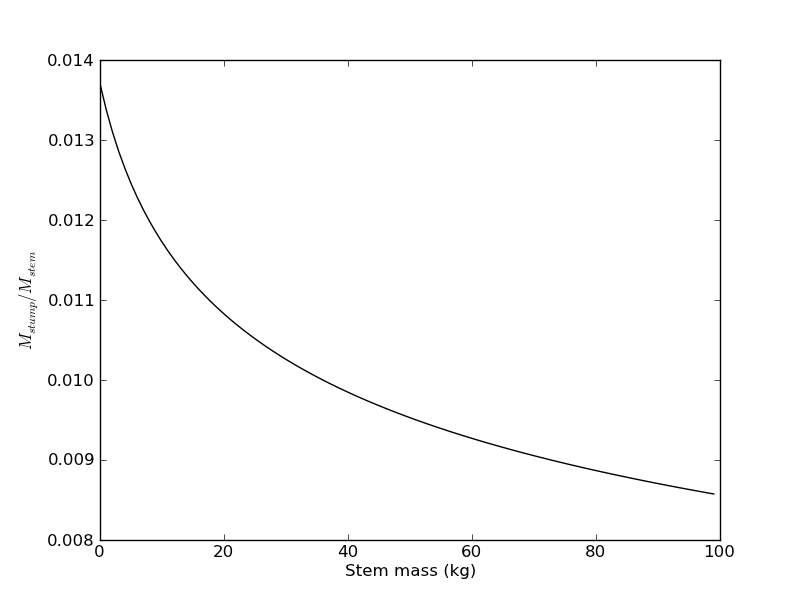
\includegraphics[width=0.5\textwidth]{nlm_stump.png}
%     \caption{Stump to stem volume ratio as a function of stem volume}
%     \label{fig:stump_vol}
%     \end{figure}
% Coefficients used in calculating stump volume as a function of total stem volume were found to be $a=0.0179877356445$ and $b=-0.169054308617$.


% \subsubsection{Predictions}

% The \ac{ahb} project uses the above model to develop an estimate of
% the potential yield of poplar throughout the study area.  Potential
% yield maps only take into consideration the climatic, environmental
% and phenological aspects.  They do not include the technical
% considerations of the technical feasibility of poplar as a crop.
% However, because management regimes effect poplar growth rates over
% the period of the rotation different harvesting patterns are included
% in the potential growth models.  The two practices considered were 12
% year cycled harvesting, and 4 four year coppicing cycles.

% The potential growth model implemented the \ac{3pg} forest growth
% model over the study area, by implementing the \ac{3pg} model within a
% \ac{GIS}.  \ac{3pg} modeled the growth of the poplar over a 12 year
% cycle, ether with or without the coppicing cycles.  

% Table~\ref{tab:3pg-grids} shows the required input grid parameters for
% the \ac{3pg} model.  In addition, the model requires a number of other
% parameterizations, primarily for the modeling of the forest. Table

% \begin{table}[!ht]
% \caption{
% \textbf{Modeling Grids}}
% \begin{tabular}{|c|c|c|}
% \hline
% Parameter & Units & Source \\
% \hline
% elevation & \meter & \\
% \hline
% precipitation & \milli\meter & \\
% \hline
% temperature & \celsius & \cite{prism-temp} \\
% \hline
% humidity & \unit{\%}  & \\
% \hline
% radiation & \mega\joule\per\squaremetre\usk\dday &  \\
% \hline
% sub-freezing days & \dday  & \\
% \hline
% \end{tabular}
% \begin{flushleft}The table shows the data sources used for the
%   modeling of the potential Growth model for poplar.
% \end{flushleft}
% \label{tab:3pg-grids}
%  \end{table}


% Do NOT remove this, even if you are not including acknowledgments
\section*{Acknowledgments}
This project was funded by the USDA's Advanced Hardwood Biofuels for
the Pacific Northwest project, Number \#.

%\section*{References}
% The bibtex filename
\bibliography{ahb-pnw}

\section*{Figure Legends}

Move Figures here at the end.

\section*{Tables}

Move Table here at the end.

%% \begin{table}[!ht]
%% \caption{
%% \textbf{Title}}
%% \begin{tabular}{|c|c|c|}
%% table information
%% \end{tabular}
%% \begin{flushleft}Caption
%% \end{flushleft}
%% \label{tab:}
%%  \end{table}

\end{document}

% LocalWords:  cellulosic biofuel feedstocks parameterized feedstock
% LocalWords:  Coppicing coppicing coppiced timestep coppice Bioenergy
% LocalWords:  Geospatial parameterize Biofuels resprouts
